
\subsection{Interfata de administrare a sistemului 'Cron'}

Interfata de administrare a sistemului de executie a operatiilor asincrone
permite vizualizarea tuturor operatiilor de acest tip, a consecintelor
acestora, precum si adaugarea si modificarea actiunilor existente. 

Trebuie mentionat insa ca orice actiune asincrona depinde de existenta
unei clase java care sa o implementeze. Astfel, introducerea unei
noi actiuni va trebui sa se bazeze exclusiv pe clasele deja implementate
in server. 


\subsubsection{Ecranul principal }

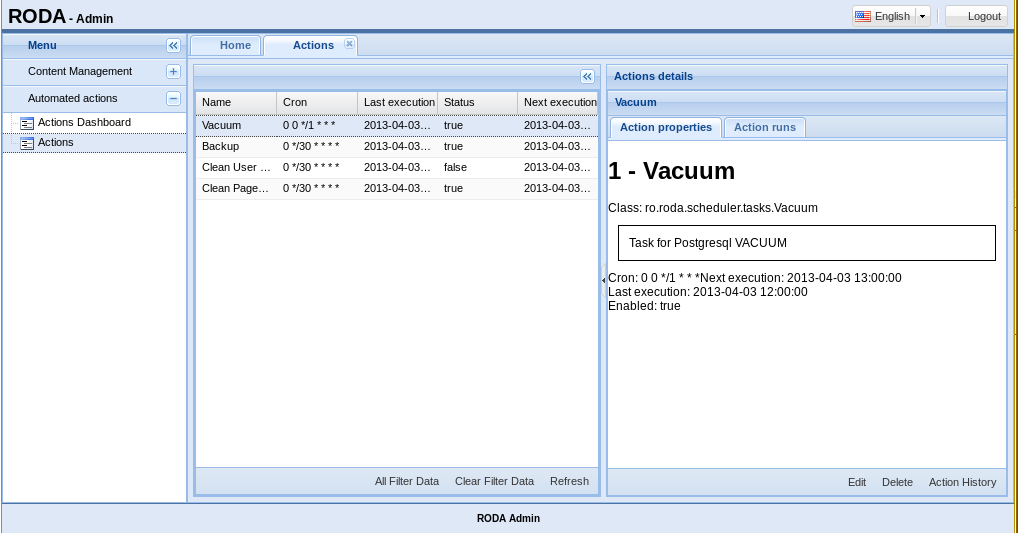
\includegraphics[width=\textwidth]{actionsview}

Ecranul principal contine doua panouri. Panoul din stanga prezinta
o lista a tuturor actiunilor din baza de date, active sau nu iar panoul
din dreapta prezinta detaliile actiunii selectate in panoul din stanga. 

Lista operatiilor contine urmtoarele informatii: 
\begin{itemize}
\item \textbf{Numele actiunii}:, un simplu nume utilizat la identificarea
actiunii 
\item \textbf{Cron:} un sistem abreviat de notare a programarii executiilor
recurente 
\item \textbf{Last execution}: momentul ultimei executari a actiunii 
\item \textbf{Active}: true pentru operatiile active, false pentru cele
care nu se executa
\end{itemize}
Panoul din dreapta poate de asemenea sa afiseze toate executiile actiunii
curente cu rezultatele acestora: 

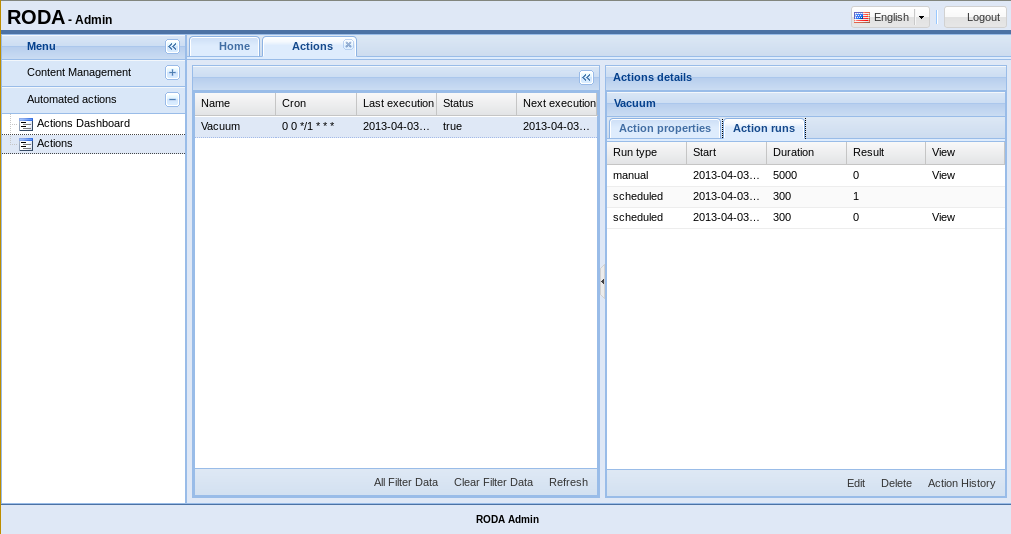
\includegraphics[width=\textwidth]{actionsview-runs}

Rezultatele unei executii sunt urmatoarele: 
\begin{itemize}
\item \textbf{Run type:} modul in care a fost executata actiunea in acel
moment. O actiune poate fi executata fie automat, conform programarii,
de catre server, fie manual, in afara programului, prin intermediul
interfetei. 
\item \textbf{Start:} momentul in care a inceput executia actiunii 
\item \textbf{Duration:} durata executiei 
\item \textbf{Result:} rezultatul operatiunii, 0 daca a general o eroare
sau 1 daca s-a executat cu succes. 
\end{itemize}
In cazul in care una dintre executii a generat o eroare, aceasta poata
fi inspectata intr-o fereastra speciala apelabila prin optiunea view
din ultima coloana: 

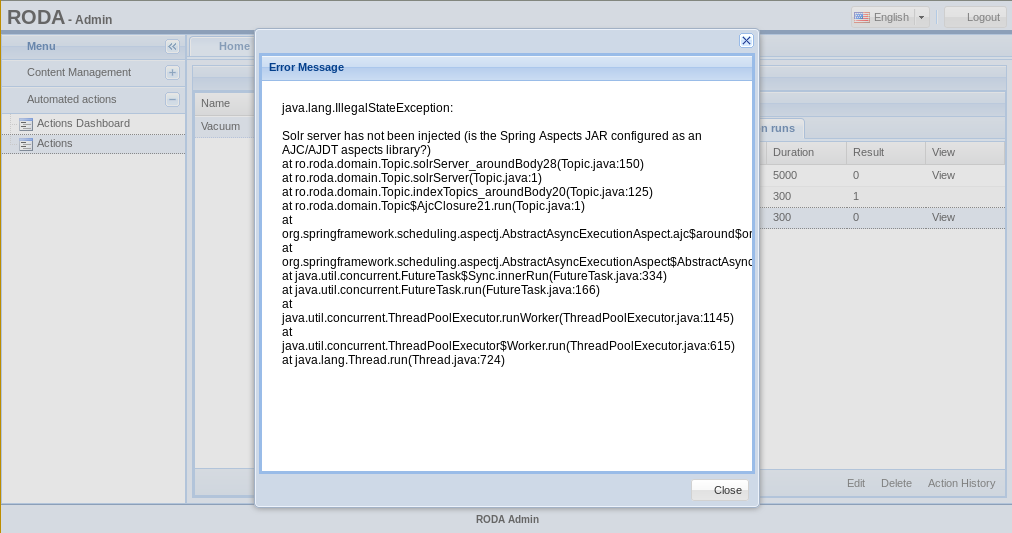
\includegraphics[width=\textwidth]{actionsview-errorview}

Panoul din stanga poate fi redus, pentru a putea vedea mai bine detaliile
operatiunii curente, in situatia in care se foloseste un monitor cu
rezolutie mica: 

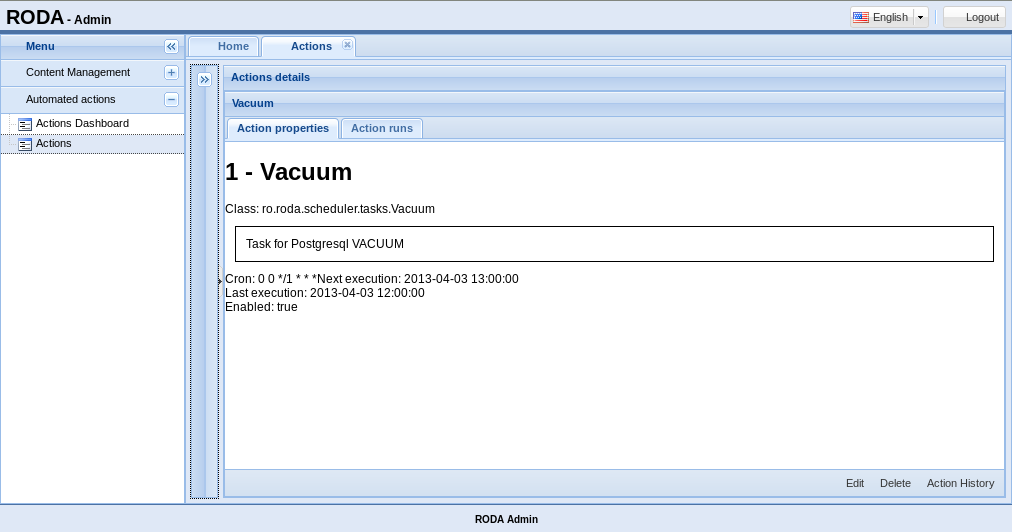
\includegraphics[width=\textwidth]{actionsview-indexcollapsed}

Panoul din stanga ofera de asemenea o serie de instrumente utile,
cum ar fi de exemplu modalitati de filtrare a rezultatelor: 

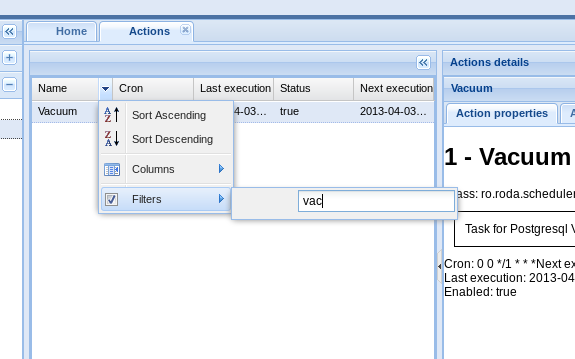
\includegraphics[width=\textwidth]{actionsview-filters}

Operatiunea curenta poate fi modificata prin utilizarea meniului contextual
disponibil pentru oricare dintre actiunile din lista: 

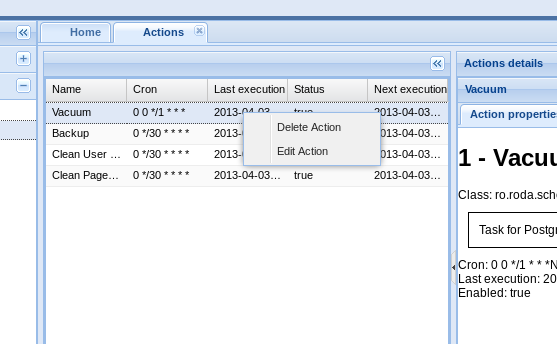
\includegraphics[width=\textwidth]{actionsview-menu}

Fereastra de editare, identica cu cea de adaugare a unei actiuni este
urmatoarea: 

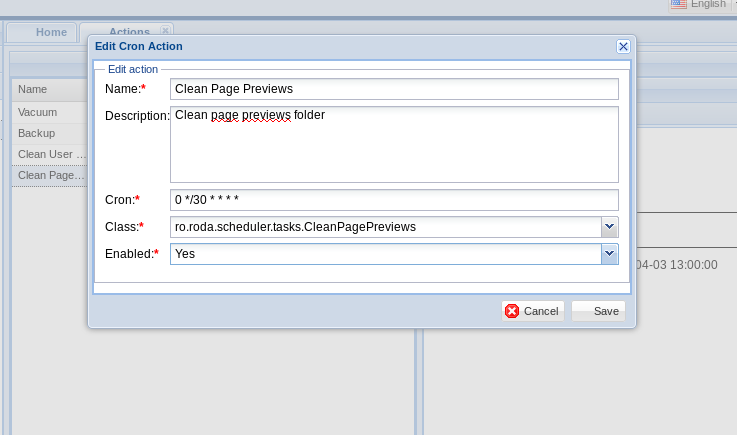
\includegraphics[width=\textwidth]{cronedit}
